\section{State of Art}

\subsection{Undirected graphs}

\paragraph{}
Undirected graphs are mathematical objects composed of a set of vertices $V$
and a set of edges $E$ and are noted $G = (V,E)$.

\paragraph{}
Also called nodes, vertices are mathematical objects which might virtually
represent anything, a vertices is usually noted $v$.

\paragraph{}
Edges are an unordered pair of vertices noted $e = (u,v)$. Edges might
contain twice the same vertex, in this case, the edge is called a {\em loop}.

\begin{figure}[!h]
  \begin{center}
    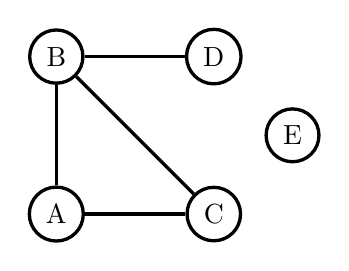
\begin{tikzpicture}[scale=0.5]
  \node[draw,circle, very thick] (A) at (2,0) {A};
  \node[draw,circle, very thick] (B) at (2,4) {B};
  \node[draw,circle, very thick] (C) at (6,0) {C};
  \node[draw,circle, very thick] (D) at (6,4) {D};
  \node[draw,circle, very thick] (E) at (8,2) {E};
  \draw[very thick] (A) -- (B);
  \draw[very thick] (B) -- (D);
  \draw[very thick] (C) -- (B);
  \draw[very thick] (C) -- (A);
\end{tikzpicture}

  \end{center}
  \caption{An undirected simple graph with 5 vertices and 4 edges}
\end{figure}

\subsubsection{Fundamentals notations}

\paragraph{Graph Size :}
The size of a graph is the number of edges it contains and is noted
$m = |E|$.

\paragraph{Graph order :}
The order of a graph is the number of vertices it contains and is noted
$n = |V|$.

\paragraph{Vertex degree :}
The degree of a vertex is equal to the number of edges incident to it, loops
are counted twice.

\paragraph{}
A path of length $n$ is a sequence of alternated vertices and edged, noted
$P = \{v_0, e_1, v_1, e_2, ..., e_n, v_n\}$ such as :
$\forall i \in \{1,2, ..., n\}, e_i = \{v_i, v_{i-1}\}$. If $v_0 = v_n$, $P$ is
a cycle.

\begin{figure}[!h]
  \begin{center}
    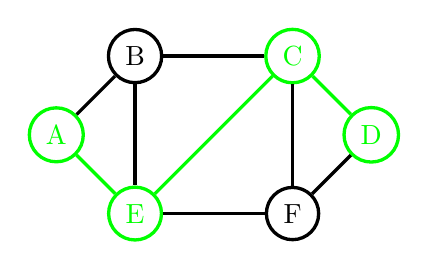
\begin{tikzpicture}[scale=0.5]
  \node[draw,circle, very thick, color=green] (A) at (0,2) {A};
  \node[draw,circle, very thick] (B) at (2,4) {B};
  \node[draw,circle, very thick, color=green] (C) at (6,4) {C};
  \node[draw,circle, very thick, color=green] (D) at (8,2) {D};
  \node[draw,circle, very thick, color=green] (E) at (2,0) {E};
  \node[draw,circle, very thick] (F) at (6,0) {F};
  \draw[very thick] (A) -- (B);
  \draw[very thick, color=green] (A) -- (E);
  \draw[very thick] (B) -- (C);
  \draw[very thick] (B) -- (E);
  \draw[very thick, color=green] (C) -- (D);
  \draw[very thick, color=green] (C) -- (E);
  \draw[very thick] (C) -- (F);
  \draw[very thick] (D) -- (F);
  \draw[very thick] (E) -- (F);
\end{tikzpicture}

  \end{center}
  \caption{A path of length 4}
\end{figure}


\subsubsection{Types of graphs}

\paragraph{Tree}
A tree is an undirected graph without cycles,

\begin{figure}[!h]
  \begin{center}
    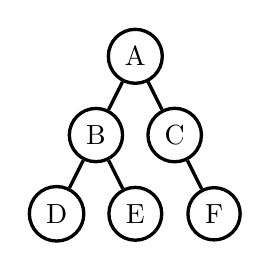
\begin{tikzpicture}[scale=0.5]
  \node[draw,circle, very thick] (A) at (2,4) {A};
  \node[draw,circle, very thick] (B) at (1,2) {B};
  \node[draw,circle, very thick] (C) at (3,2) {C};
  \node[draw,circle, very thick] (D) at (0,0) {D};
  \node[draw,circle, very thick] (E) at (2,0) {E};
  \node[draw,circle, very thick] (F) at (4,0) {F};
  \draw[very thick] (A) -- (B);
  \draw[very thick] (A) -- (C);
  \draw[very thick] (B) -- (D);
  \draw[very thick] (B) -- (E);
  \draw[very thick] (C) -- (F);
\end{tikzpicture}

  \end{center}
  \caption{A tree}
\end{figure}

\paragraph{Spanning Tree}
A tree is a spanning tree of a graph G if it includes every vertex of G and is a subgraph of G (every edge in the tree belongs to G).

\begin{figure}[!h]
  \begin{center}
    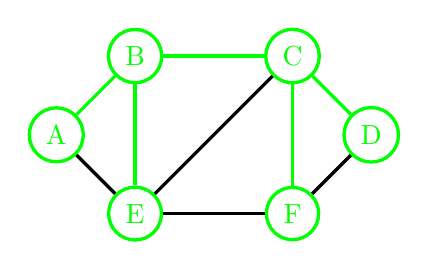
\begin{tikzpicture}[scale=0.5]
  \node[draw,circle, very thick, color=green] (A) at (0,2) {A};
  \node[draw,circle, very thick, color=green] (B) at (2,4) {B};
  \node[draw,circle, very thick, color=green] (C) at (6,4) {C};
  \node[draw,circle, very thick, color=green] (D) at (8,2) {D};
  \node[draw,circle, very thick, color=green] (E) at (2,0) {E};
  \node[draw,circle, very thick, color=green] (F) at (6,0) {F};
  \draw[very thick, color=green] (A) -- (B);
  \draw[very thick] (A) -- (E);
  \draw[very thick, color=green] (B) -- (C);
  \draw[very thick, color=green] (B) -- (E);
  \draw[very thick, color=green] (C) -- (D);
  \draw[very thick] (C) -- (E);
  \draw[very thick, color=green] (C) -- (F);
  \draw[very thick] (D) -- (F);
  \draw[very thick] (E) -- (F);
\end{tikzpicture}

  \end{center}
  \caption{A spanning tree}
\end{figure}


\subsubsection{Subgraphs}

\subsubsection{Cuts}



\subsubsection{Connectivity}
\paragraph{Connectivity}
A graph  is {\em connected} if $\forall u,v \in V$ a path exists from $u$
to $v$. Otherwise, the graph is {\em unconnected}

\paragraph{k-connectivity}
A graph with a least two vertices is k-connected if, for every pair of vertices, there is at least k vertex disjoint paths between these vertices.

A graph is k-connected if the smallest subset which disconnect the graph if you delete it is of size k.

\begin{figure}[!h]
  \begin{center}
    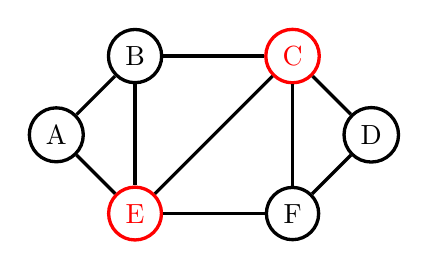
\begin{tikzpicture}[scale=0.5]
  \node[draw,circle, very thick] (A) at (0,2) {A};
  \node[draw,circle, very thick] (B) at (2,4) {B};
  \node[draw,circle, very thick, color=red] (C) at (6,4) {C};
  \node[draw,circle, very thick] (D) at (8,2) {D};
  \node[draw,circle, very thick, color=red] (E) at (2,0) {E};
  \node[draw,circle, very thick] (F) at (6,0) {F};
  \draw[very thick] (A) -- (B);
  \draw[very thick] (A) -- (E);
  \draw[very thick] (B) -- (C);
  \draw[very thick] (B) -- (E);
  \draw[very thick] (C) -- (D);
  \draw[very thick] (C) -- (E);
  \draw[very thick] (C) -- (F);
  \draw[very thick] (D) -- (F);
  \draw[very thick] (E) -- (F);
\end{tikzpicture}

  \end{center}
  \caption{A 2-connected graphe}
\end{figure}


